\documentclass{standalone}
\usepackage{tikz}

\begin{document}

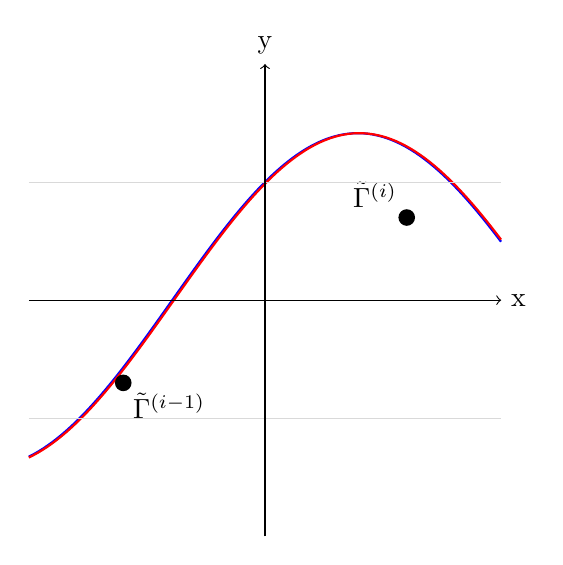
\begin{tikzpicture}[scale=1.5]
    % Define the domain for the curves
    \def\xmin{-2}
    \def\xmax{2}
    
    % Draw the curve \tilde{\Gamma}^{(i)}
    \draw[blue, thick] plot[domain=\xmin:\xmax, samples=100] ({\x},{sin(\x r) + cos(\x r)});
    
    % Draw the curve \tilde{\Gamma}^{(i-1)}
    \draw[red, thick] plot[domain=\xmin:\xmax, samples=100] ({\x},{sin(\x r - pi/4) + cos(\x r - pi/4)});
    
    % Mark the intersection points
    \fill[black] (1.2, 0.7) circle (2pt);
    \fill[black] (-1.2, -0.7) circle (2pt);
    
    % Label the curves
    \node[above left] at (1.2, 0.7) {\(\tilde{\Gamma}^{(i)}\)};
    \node[below right] at (-1.2, -0.7) {\(\tilde{\Gamma}^{(i-1)}\)};
    
    % Add grid and axis labels
    \draw[gray!30] (\xmin,-1) -- (\xmax,-1);
    \draw[gray!30] (\xmin,1) -- (\xmax,1);
    \draw[->] (\xmin,0) -- (\xmax,0) node[right] {x};
    \draw[->] (0,\xmin) -- (0,\xmax) node[above] {y};
\end{tikzpicture}

\end{document}